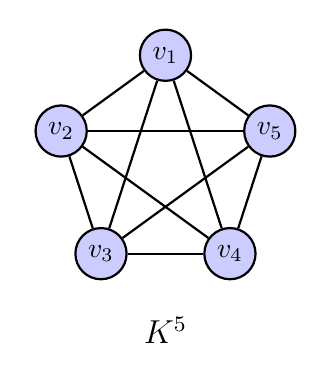
\begin{tikzpicture}[
  baseline=0pt,
  scale=0.7,
  vnode/.style={circle, draw=black, fill=blue!20, thick, inner sep=0pt, minimum size=6.5mm},
  edge/.style={thick, draw=black}
]
  \useasboundingbox (-2.5,-3.4) rectangle (2.5,2.3);

  % v1 en y=1.8, vértices inferiores en y=-1.8
  \node[vnode] (v1) at ([yshift=-0.19cm]90:1.99) {$v_1$};
  \node[vnode] (v2) at ([yshift=-0.19cm]162:1.99) {$v_2$};
  \node[vnode] (v3) at ([yshift=-0.19cm]234:1.99) {$v_3$};
  \node[vnode] (v4) at ([yshift=-0.19cm]306:1.99) {$v_4$};
  \node[vnode] (v5) at ([yshift=-0.19cm]18:1.99) {$v_5$};

  % Aristas
  \draw[edge] (v1) -- (v2); \draw[edge] (v1) -- (v3); \draw[edge] (v1) -- (v4); \draw[edge] (v1) -- (v5);
  \draw[edge] (v2) -- (v3); \draw[edge] (v2) -- (v4); \draw[edge] (v2) -- (v5);
  \draw[edge] (v3) -- (v4); \draw[edge] (v3) -- (v5);
  \draw[edge] (v4) -- (v5);

  % Etiqueta
  \node[font=\large] at (0,-3.2) {$K^5$};
\end{tikzpicture}
